\documentclass{beamer}

\usepackage[utf8]{inputenc}
\usepackage{default}
\usepackage[OT4]{polski}
\usepackage[normalem]{ulem}
\usepackage{color}
\usepackage{graphicx}
\usepackage{tikz}
\usetheme{Warsaw}

\tikzstyle{line} = [draw, -latex]
\tikzstyle{path} = [draw, -latex, style={decorate,decoration={snake}}]
\tikzstyle{state} = [circle,draw=black,minimum size=0.9cm]
\tikzstyle{finish_state} = [circle,draw=black,double=white,double distance=1pt,minimum size=0.9cm]
\usetikzlibrary{shapes,arrows,automata,decorations.pathmorphing}

\begin{document}
	\begin{frame}
		\frametitle{ZPP -- NianioLang}
		Cotygodniowa prezentacja
		
		02.11.2017
	\end{frame}
	
	\begin{frame}
		\frametitle{Wprowadzenie do kompilatora NianioLanga}
		\begin{itemize}
		 \item Podstawowe pojęcia
		 \begin{itemize}
		  \item AST -- Abstract Syntax Tree
		  \item nlasm -- kod pośredni NianioLanga, ciąg rozkazów zbliżony do kodu maszynowego
		 \end{itemize}
		 \pause
		 \item System typów
		 \begin{itemize}
		  \item Typy proste, tablice, hashe, rekordy, warianty
		  \item Typy definiowane poprzez funkcje: \texttt{ptd::arr(ptd::sim())}
		  \item \textbf{Obecnie informacja o typach jest tracona przy kompilacji}
		 \end{itemize}
		\end{itemize}
	\end{frame}
	
	\begin{frame}
	 \frametitle{Wysokopoziomowe spojrzenie na kompilator}
	\tikzset{loop below/.style={min distance=10mm,in=315,out=235,looseness=8}}
	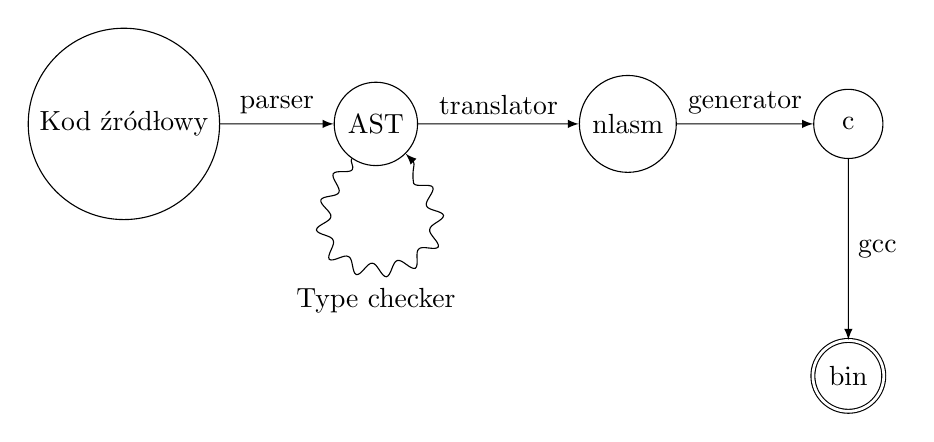
\begin{tikzpicture}
			[scale=.8,auto=left]
			\node [state] (src) at (1,1) {Kod źródłowy};
			\node [state] (ast) at (5,1) {AST};
			\node [state] (nlasm) at (9,1) {nlasm};
			\node [state] (c) at (12.5,1) {c};
			\node [] (type_checker) at (5,-1.8) {Type checker};
			\node [finish_state] (bin) at (12.5,-3) {bin};
			\path [line] (src) to[left] node[auto] {parser} (ast);
			\path [line] (ast) to[left] node[auto] {translator} (nlasm);
			\path [line] (nlasm) to[left] node[auto] {generator} (c);
			\path [line] (c) to[left] node[auto] {gcc} (bin);
			\path [path] (ast) to[out=235,in=315,distance=3cm] (ast);
		\end{tikzpicture}
		\end{frame}
	
	\begin{frame}
		\frametitle{Co miało być zrobione}
		\begin{itemize}
		 \item Stworzenie strony projektu i opisanie początkowych ustaleń 
		 \item Skonfigurowanie Continuous Integration
		 \item Wyznaczenie pierwszych zadań
		\end{itemize}
	\end{frame}
	
	\begin{frame}
		\frametitle{Stworzenie strony projektu}
		\begin{itemize}
			\item\textcolor{green}{Zrobione}
			\begin{itemize}
				\item https://jbujak.github.io/nl-zpp/ 
			\end{itemize}
		\end{itemize}
	\end{frame}
	
	\begin{frame}
		\frametitle{Przygotowanie wsparcia dla Continuous Integration}
		\begin{itemize}
			\item\textcolor{yellow}{Częściowo zrobione}
			\begin{itemize}
				\item Jest budowanie projektu jednym poleceniem
				\item Są testy automatyczne przy każdym pełnym budowaniu projektu
				\item Pozostało skonfigurowanie Travisa
			\end{itemize}
		\end{itemize}
	\end{frame}
	
	\begin{frame}
		\frametitle{Wyznaczenie i wykonanie pierwszych zadań}
		\begin{itemize}
			\item \textcolor{green}{Zrobione}
			\begin{itemize}
				\item Oznaczenie w drzewie AST funkcji, które definiują typ -- Michał Borkowski
				\item Przeniesienie tej informacji do nlasm -- Marek Puzyna
				\item Wygenerowanie pustej struktury dla każdego zdefiniowanego typu -- Jakub Bujak
				\item Przygotowanie testów sprawdzających powyższe -- Marian Dziubiak
			\end{itemize}
		\end{itemize}
		\pause
		\textbf{Wszystkie zadania zostały wykonane}
	\end{frame}
	
	\begin{frame}
		\frametitle{Przygtowanie środowiska pracy}
		\begin{itemize}
			\item\textcolor{green}{Zrobione}
			\begin{itemize}
				\item Repozytorium kodu: git
				\item Repozytorium zadań i błędów: GitHub issues
				\item Wspieranie code review:
					\begin{itemize}
					\item Push block na masterze
					\item Możliwość mergowania pull requesta dopiero po pomyślnym review
					\end{itemize}
				\item Wspieranie komunikacji grupy: GitHub wiki
				\item Dostęp do powyższych: github.com/jbujak/nl-zpp
			\end{itemize}
		\end{itemize}
	\end{frame}
	
	\begin{frame}
		\frametitle{Lista zadań i plany na najbliższy tydzień}
		\begin{itemize}
			\item{Na najbliższy tydzień}
			\begin{itemize}
				\item{\textbf{Dokończyć konfigurację Travisa}}
				\item{\textbf{Dodać kompilację intów NianioLanga do intów C}}
				\item{\textbf{Dodać obsługę intów w type checkerze}}
			\end{itemize}
			\item{Do zrobienia ogólnie}
			\begin{itemize}
				\item{Przystosować type checker do współpracy z resztą nowych typów}
				\item{Umożliwić kompilację tablic, rekordów i reszty typów prostych do struktur C}
				\item{Zaimplementować podstawowe operacje na skompilowanych strukturach}
			\end{itemize}
		\end{itemize}
	\end{frame}
\end{document}
